\subsection{ITS}
\label{recoEPN:ITS}

In opposite to Run1 situation, where most of the tracks in the ITS are found as prolongation
of TPC tracks, in Run3 the TPC itself needs ITS tracks in order to perform final calibration of
the space charge distortions. Therefore, a standalone tracking in the ITS needs to be performed.
The principal requirement to the code used for ITS tracking is the speed, since at least the part
of reconstuction should be performed in real time.
The algorithm that is currently under study is based on a Cellular Automaton (CA) (see 
Alice ITS TDR \cite{refITSTDR} and \cite{refCA1, refCA2}). Since at the moment no working code exists 
for the ALICE ITS, for the estimates of its performance we have to rely on the benchmarking done by the
CBM collaboration for their Silicon tracker made of 8 planes of microstrips. 
The reconstruction consisted of three passes by the algorithm, the first two corresponding to a search of 
high and low \pt tracks converging to vertex region and the third one for the secondary tracks (w/o requirement
of the convergence to the vertex).
The estimated reconstruction efficiency is shown on Fig.~\ref{fig:ITSreceffCBM} (left) 
for single central Au-Au collision as function of the track momentum and (right) as function of the multiplicity
(created by piling up the space points from many minumum bias collisions). 

\begin{figure}[h]
\centering
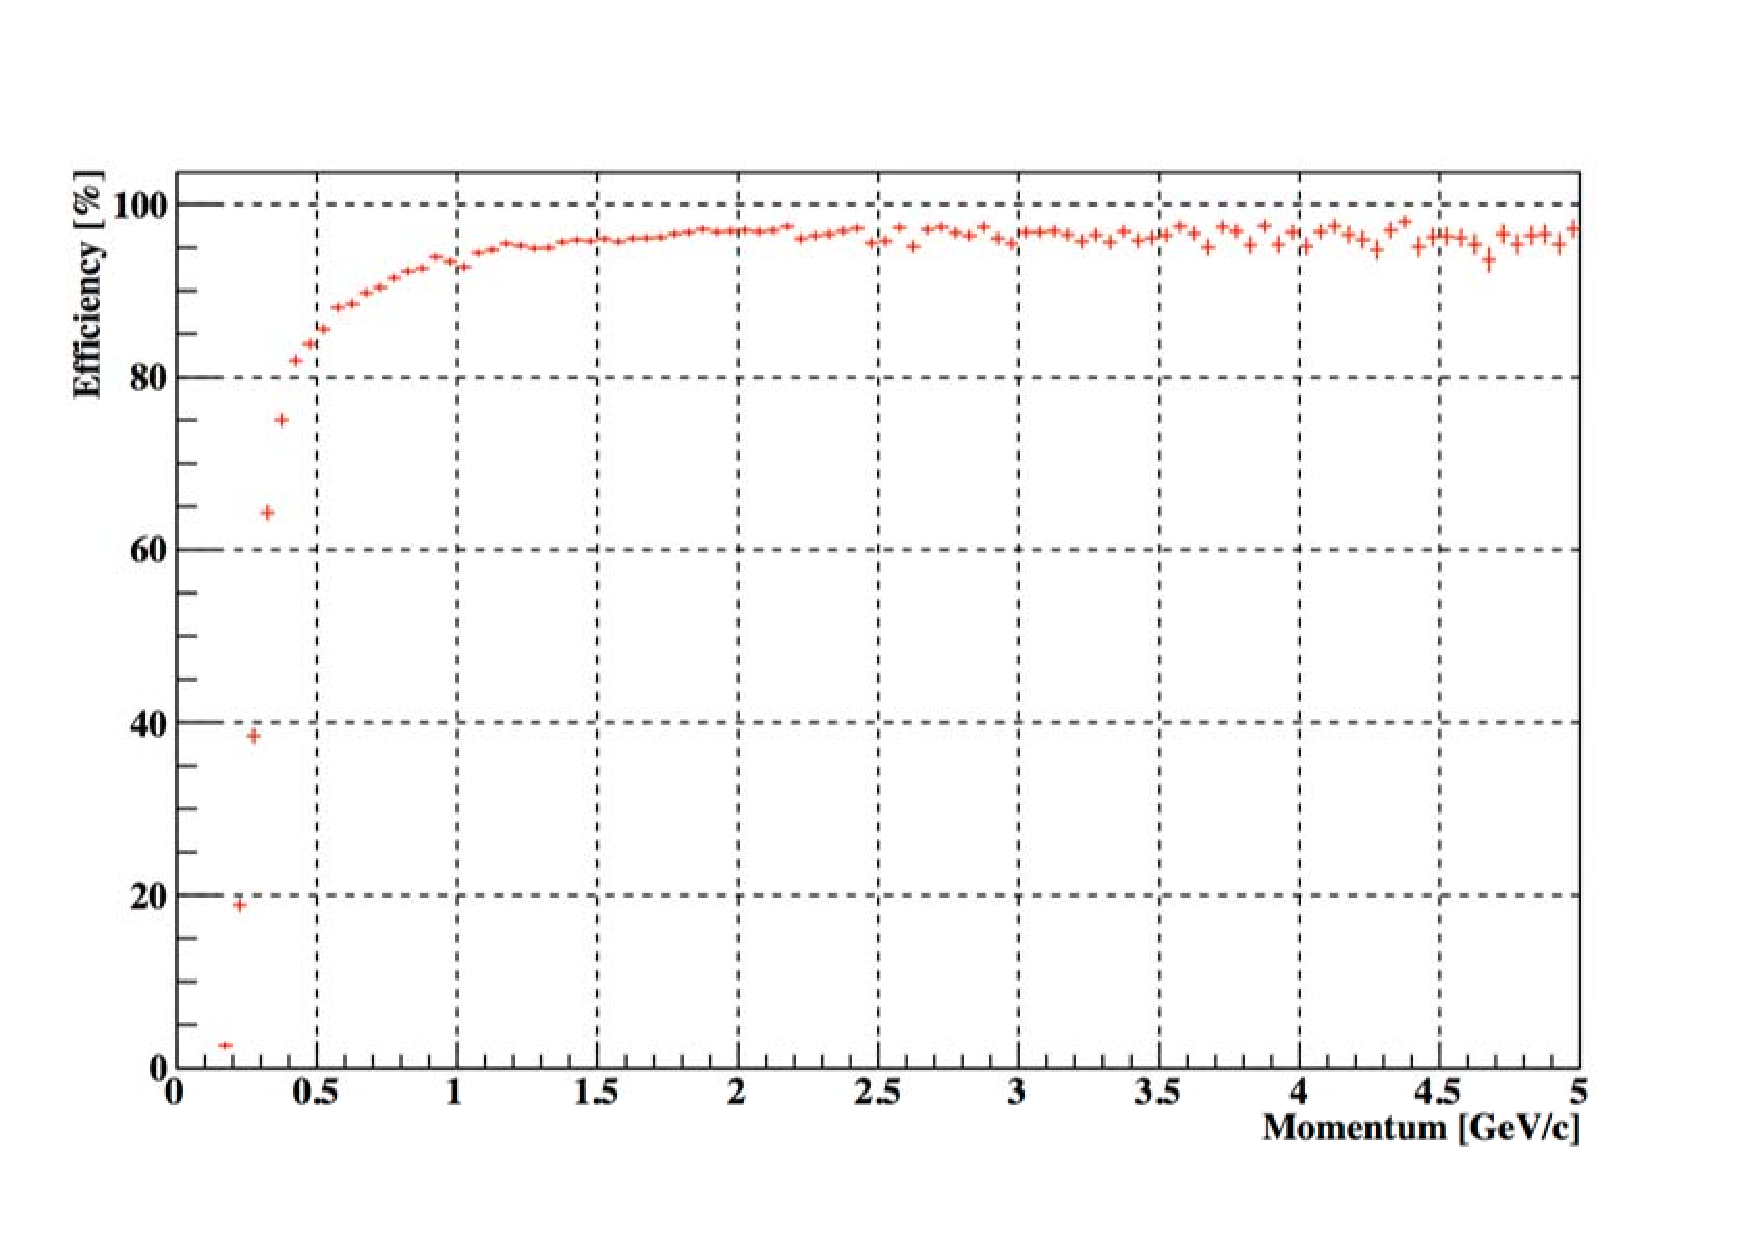
\includegraphics[width=0.48\textwidth]{ITS/IK_CBMeff.pdf}
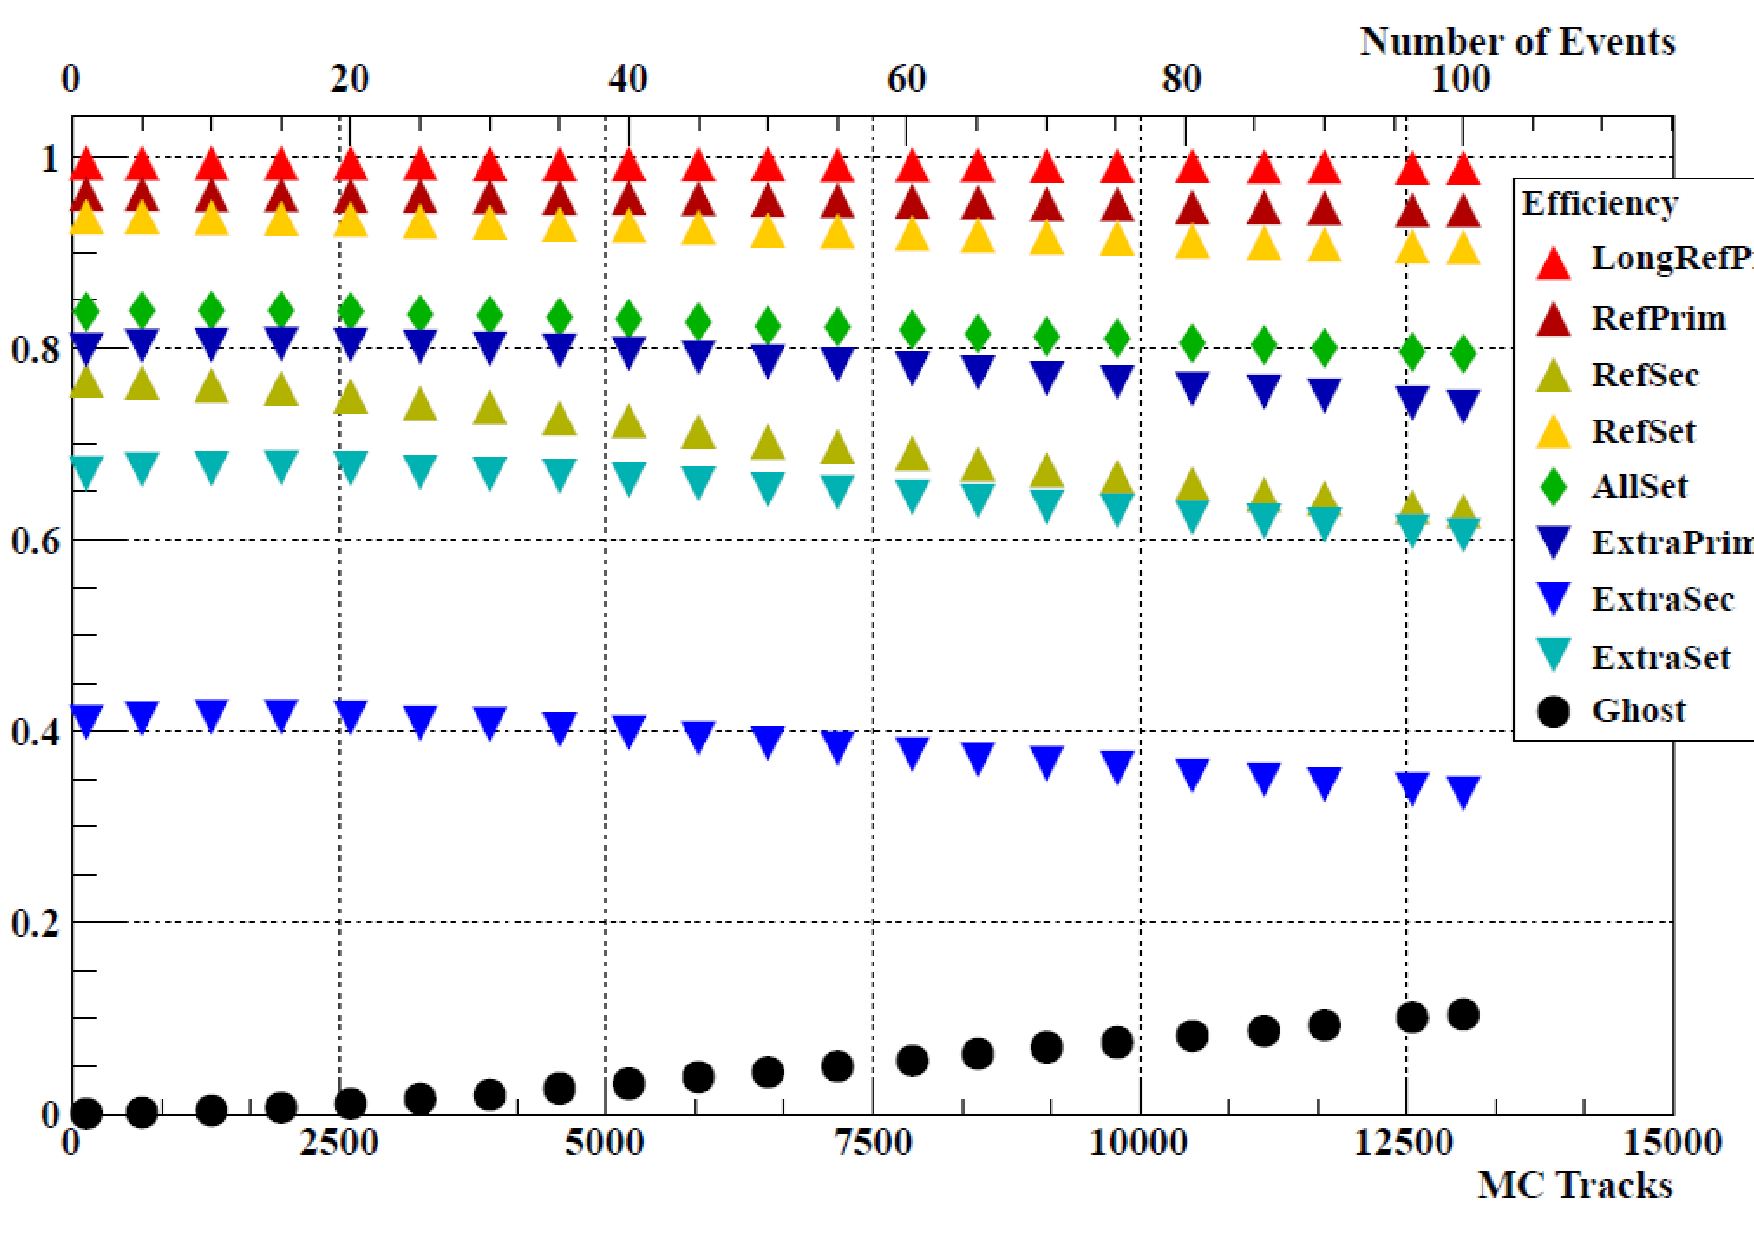
\includegraphics[width=0.48\textwidth]{ITS/IK_CBMeffmult.pdf}
\caption{\label{fig:ITSreceffCBM} 
Reconstruction efficiency of CBM CA tracker for single central Au-Au event (left)
and as a function of multiplicity obtained by piling up multiple collisions (right).
}
\end{figure}

Fig.~\ref{fig:ITSrecotimeCBM} shows the reconstruction time as a function of the multiplicity 
in the detector acceptance, performed on the single core of the Intel E7-4860 at 2.27 GHz processor. 
The multiplicities expected in the Alice ITS
for central \pbpb collision and in the single ITS readout cycle of 30\ums at 50 kHz interaction rate are shown
by the red bars. The timing of $\sim$0.2 s for reconstruction of average readout cycle seen on this figure cannot
be directly applied to Alice case. First of all, CBM, being a fixed target experiment, sees in average tracks of 
higher momentum that Alice. While Alice needs to perform the tracking up to momenta (e.g. \pt) below 100~MeV/c,
the CBM reconstructed momentum spectrum stops at momentum $\sim$250 MeV/c. Given that the reconstruction of the 
low momentum tracks is most time consuming, one should expect faste reconstruction in the CBM
tracker than in the Alice ITS. As a tentative estimate we assume that the average ITS readoud cycle (with multiplicity
equivalent to that of 1.5 minimum bias \pbpb collisions at 50 kHz interaction rate) can be reconstructed in less than
1 s on a single core. 

\begin{figure}[h]
\centering
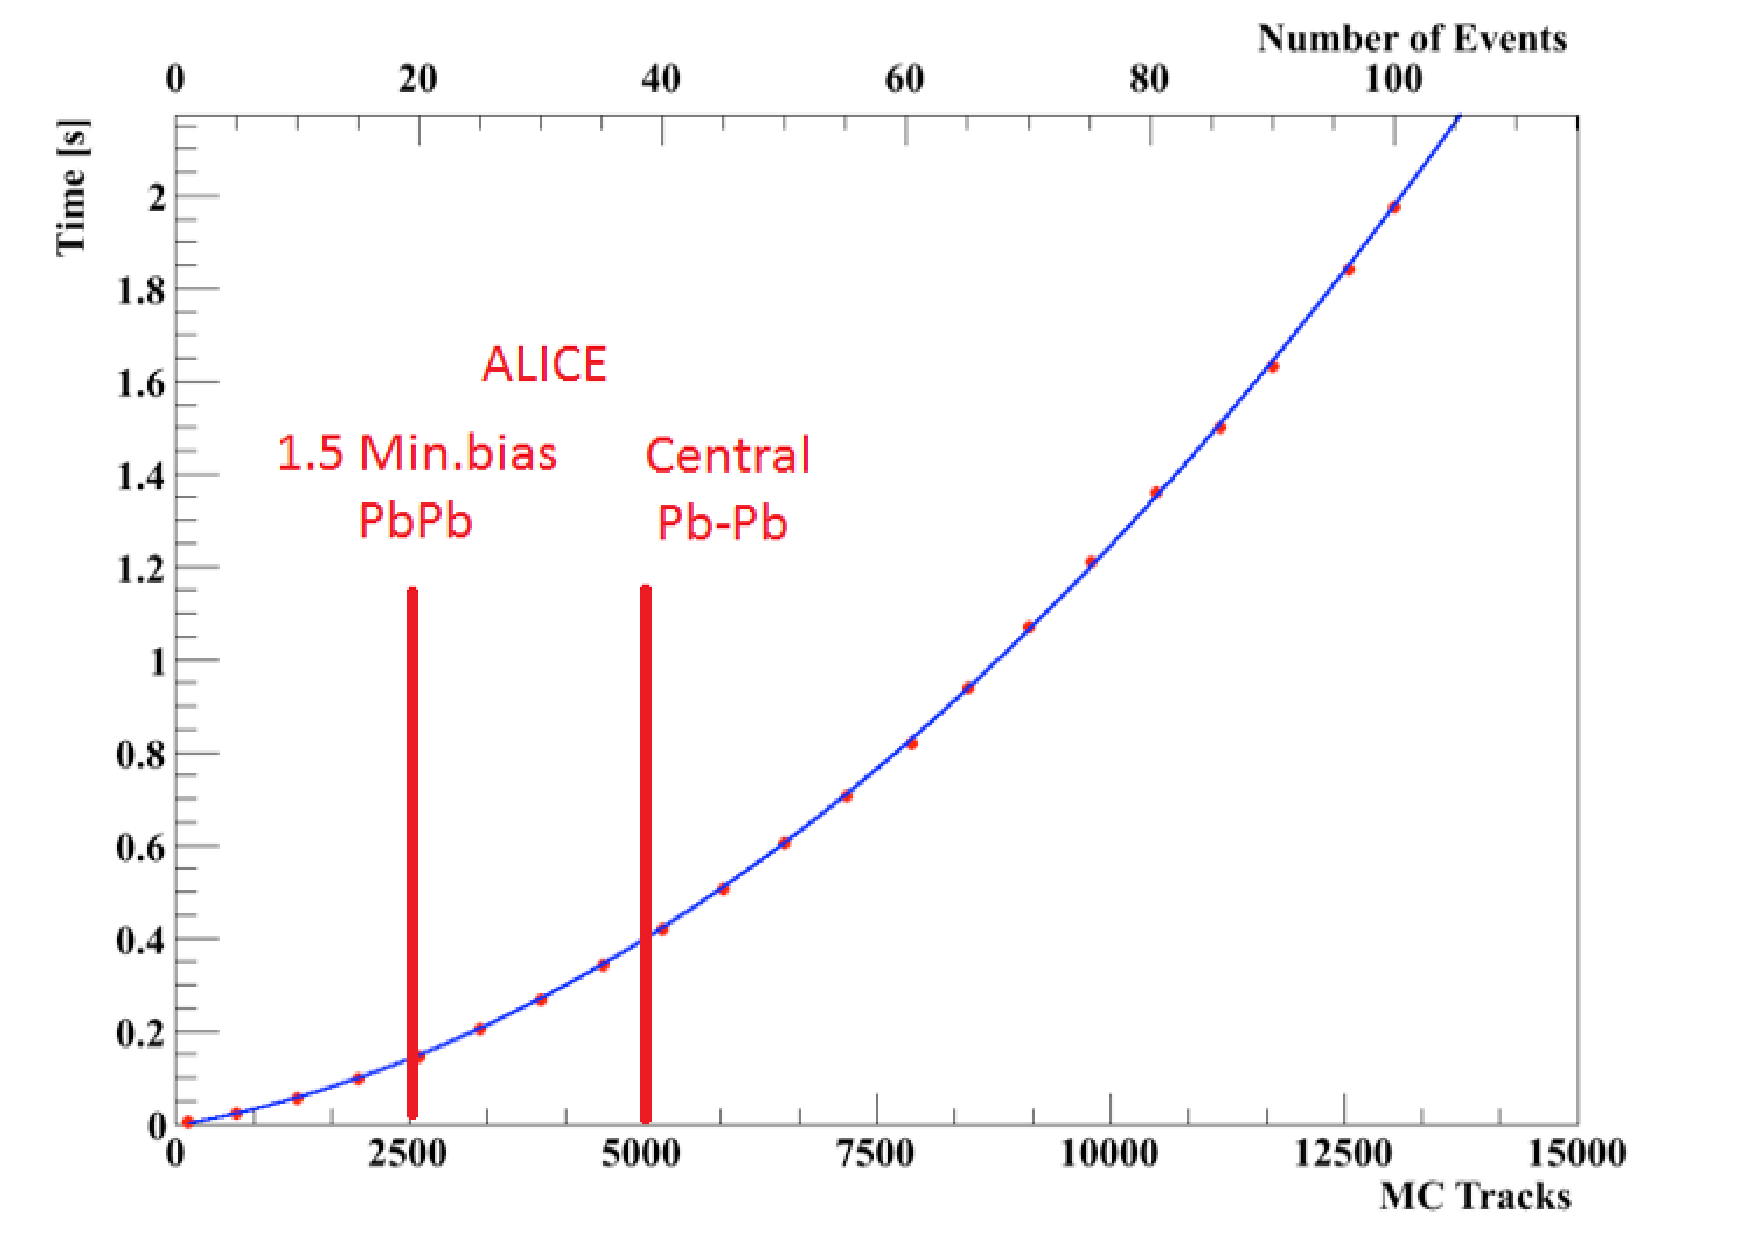
\includegraphics[width=0.80\textwidth]{ITS/IK_CBMrecotime.pdf}
\caption{\label{fig:ITSrecotimeCBM} 
Results of benchmarking for reconstruction time versus number of 
tracks in the acceptance for CBM CA tracker (on a single core of the Intel
E7-4860 at 2.27 GHz processor).
}
\end{figure}


As it was mentioned 
in Sect.~\ref{ITS:datarate}, one cannot exclude that the cluster data will be dominated by the random noise in
the pixel detectors, in which case even after the compression described in Sect.\ref{recoEPN:ITS} the rate
of the ITS cluster data will exceed 20 GB/s, factor 2 higher than the maximum target rate for storage.
Therefore, the aim of the on-line reconstrcution is not only finding the tracks in the ITS and providing a 
constraint for TPC calibration
but also the reduction of the cluster data to the level acceptable for the permanent storage. 
Approximately 50\% of clusters produced by the primary and secondary particles are not used by the 
reconstructed tracks, hence can be rejected before the storage (provided that the reconstruction reaches its
maximum efficiency). This fraction will increase even further if the cluster data are dominated by the noise,
guaranteeng the reduction of the storable data rate to acceptable level. 

In case the full reconstruction of the ITS will appear to be too slow for the real-time processing, it should be
performed either in quasi-online (i.e. data is bufferized locally on the EPN and reconstructed by the
beginning of the next fill) or the offline mode. For this scenario we are considering an alternative way of 
the cluster reduction which does not require full real-time tracking. The idea is to keep only those clusters
of the outer 5 layers (containing 95\% of noise clusters)
which can be bound to helical triplets pointing to the proximity of the interaction region. Since binding the
clusters in such triplets is a necessary step also in the CA tracker, one can consider such a data reduction
in the incomplete reconstruction as a rescue mode of the full tracking. The preliminary estimates of data
reduction by combining clusters to triplets is XXX\% and YYY\% for the scenario with $10^{-5}$ noise and 
without the noise respectively.
